\documentclass[11pt]{article}

\usepackage{a4wide}
\usepackage[utf8]{inputenc}
\usepackage[russian]{babel}
\usepackage{graphicx}
\usepackage{amsmath}
\usepackage{amsthm}
\usepackage{amssymb}
\usepackage{url}

\newtheorem{ConvexHull}{Определение}

\newcommand*{\hm}[1]{#1\nobreak\discretionary{}{\hbox{$\mathsurround=0pt #1$}}{}}
\newcommand\abs[1]{\left\lvert#1\right\rvert}
\newcommand{\scalar}[2]{\left<#1,#2\right>}

\DeclareMathOperator{\conv}{Conv}

\begin{document}
\thispagestyle{empty}

\begin{center}
\ \vspace{0cm} % WTF?! There were -3cm in example, but it worked strange.
\includegraphics[width=0.5\textwidth]{msu.eps}\\
{\scshape Московский государственный университет имени М.~В.~Ломоносова}\\
Факультет вычислительной математики и кибернетики\\
Кафедра системного анализа

\vfill
{\LARGE Отчёт по практикуму} \\
\vspace{1cm}
{\Huge\bfseries <<Эффективное написание алгоритмов>>}
\end{center}

\vspace{1cm}
\begin{flushright}
\large
\textit{Студент 315 группы}\\
В.~С.~Терёшин\\
%\vspace{5mm}
%\textit{Руководитель практикума}\\
%к.ф.-м.н., доцент П.~П.~Петров
\end{flushright}

\vfill
\begin{center}
Москва, 2013
\end{center}

\pagebreak

\section{Постановка задачи}
В данном задании по практикуму требовалось построить аналог функции \texttt{convhull} системы программирования \texttt{MATLAB},
выполняющий построение границы выпуклой оболочки множества точек.
\begin{ConvexHull}[Выпуклая оболочка]
Выпуклой оболочкой множества $X$ называется пересечение всех выпуклых множеств $Y$ таких, что $X \subseteq Y$.
\end{ConvexHull}

Функция \texttt{convhull} принимает два вектора \texttt{x} и \texttt{y} одинаковой длины, обозначающих координаты $x$ и $y$ данного множества точек, и возвращает вектор индексов точек, входящих в границу выпуклой оболочку, в порядке обхода против часовой стрелки.
Корректность работы построенной функции требовалось оценить на нескольких десятках входных данных специальным скриптом.

Кроме того, требовалось реализовать GUI, позволяющий пользователю указывать точки на координатной плоскости, а также параметры вывода информации. При этом должна допускаться коррекция ошибок.

\section{Решение задачи}
Для решения задачи использовался алгоритм быстрой оболочки. Его сложность $\underline{\mathsf{O}}(n\log{n})$.
\subsection{Описание алгоритма}
\begin{enumerate}
	\item
		Возьмём две крайние точки множества $S$ --- левую $L$ и правую $R$. Проведём прямую через них. Обозначим через $S_1$ подмножество точек, расположенных выше или на прямой через точки $L$ и $R$, а через $S_2$ --- подмножество точек, ниже или на данной прямой.
	\item
		Рассмотрим верхнее подмножество $S_1$. Выберем из него точку $P_i$, имееющую наибольшее удаление от трямой $LR$. Если таких точек несколько, выбираем ту, у которой угол $\angle P_iLR$ наибольший. Точка $P_i$ является вершиной выпуклой оболочки множества. В самом деле, если через точку $P_i$ провести прямую, параллельную прямой $LR$, то выше этой прямой не окажется ни одной точки множества $S$. Возможно, на построенной прямой окажутся другие точки, но, согласно сделанному выбору, $P_i$ из них самая левая. Точка $P_i$ не может быть представлена выпуклой комбинацией двух других точек множества $S$. Построим прямые $LP_i$ и $P_iR$. Точки, расположенные справа от обеих прямых, могут быть исключены из дальнейшего рассмотрения, поскольку они являются внутренними точками треугольника $\triangle LP_iR$, т.~е. не принадлежат границе выпуклой оболочки множества $S$.
	\item
		Теперь рассмотрим подмножество точек $S_{11}$, расположенных слева от прямой $LP_i$ или на ней, и подмножество точек $S_{12}$, расположенных слева от прямой $P_iR$ или на ней. Для каждого из этих подмножеств построим выпуклую оболочку. Выпуклая оболочка $S_1$ образуется склейкой упорядоченных списков вершин, входящих в выпуклые оболочки $S_{11}$ и $S_{12}$.
	\item
		Решаем задачу для $S_2$.
\end{enumerate}

\section{Примеры работы}
\subsection{Скриншоты}
\includegraphics[scale=0.5]{pict1.eps}
\includegraphics[scale=0.5]{pict2.eps} \newline
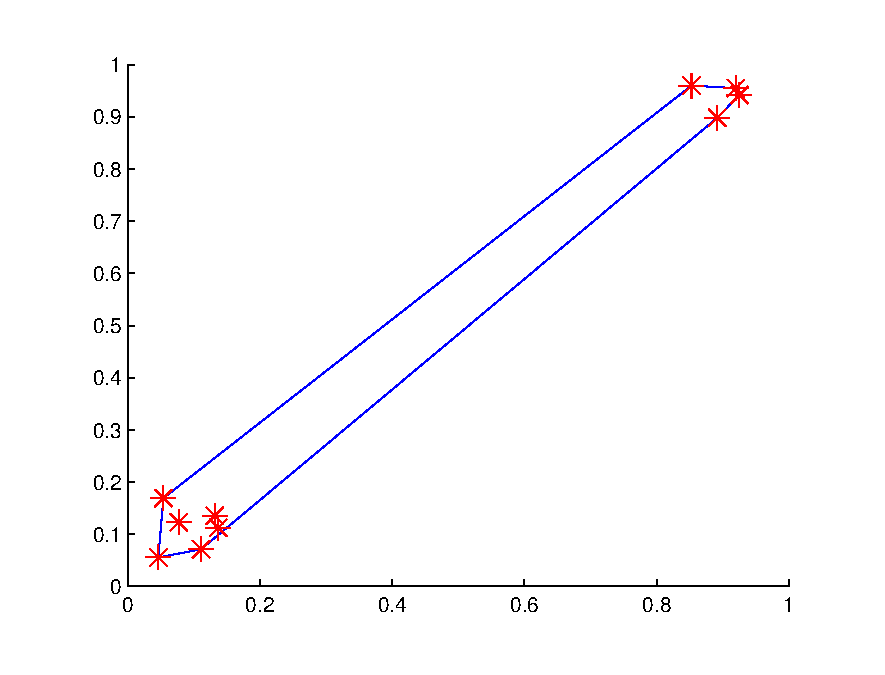
\includegraphics[scale=0.5]{pict3.eps}
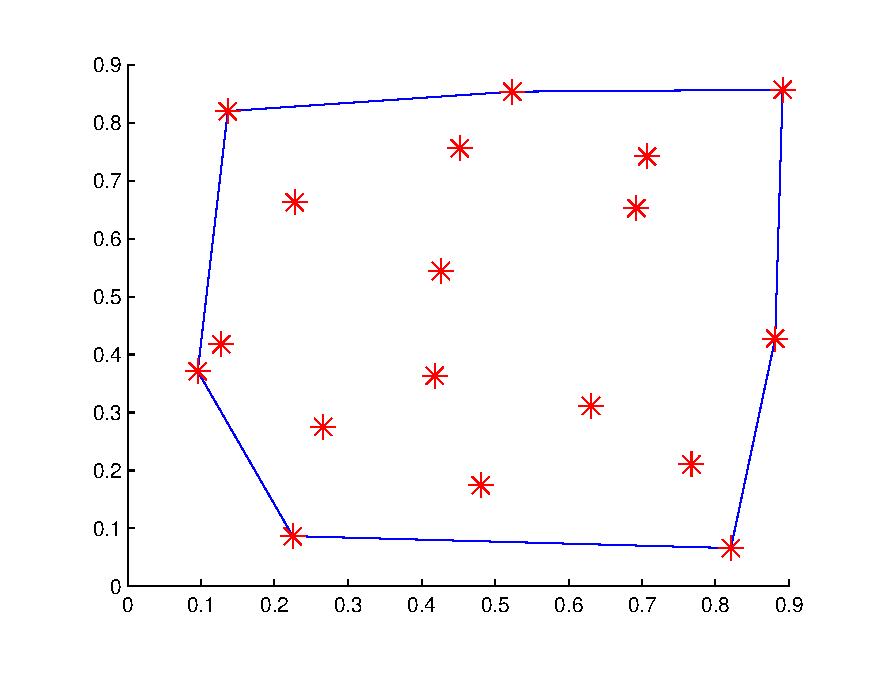
\includegraphics[scale=0.5]{pict4.eps} \newline

\subsection{Время работы}
\includegraphics[scale=0.5]{time1.eps}
\includegraphics[scale=0.5]{time2.eps}

На первом графике --- время работы функции на выборке с нормальным распределением с $a = 0,\	 \sigma = 1$, на втором --- с равномерным распределением на $[0,1]$.

Реализованный алгоритмы закономерно очень много проигрывает по времени нативному.

\section{Замечания}
Достаточно неприятным известием стала некорректность встроенной функции \texttt{convhull}. Например, на безобидном тесте, состоящем из двадцати точек, лежащих на одной прямой, \texttt{convhull} превышала допутимый размер стека. В некоторым других случаях \texttt{convhull} возвращала не совсем правильный результат (включала в ответ несколько точек на стороне выпуклого многоугольника).

\begin{thebibliography}{99}
	\bibitem{wiki} \url{http://ru.wikipedia.org/wiki/QuickHull}
	\bibitem{IAD} Дигайлова~И.~А. Лекции по \LaTeX. 2009.
\end{thebibliography}
\end{document}
